\documentclass[a4paper]{scrartcl}
\usepackage[
    fach=Geschichte,
    lerngruppe={6a},
    typ=ib,
    seitenzahlen=keine,
    loesungen=keine,
]{schule}

% Dieses Dokument gehört zu den Beispiel des LaTeX Paketes Schule und ist von den Autoren
% des Pakets erstellt worden.
%
% Das Dokument steht unter der Lizenz: Creative Commons by-nc-sa Version 4.0
% http://creativecommons.org/licenses/by-nc-sa/4.0/deed.de
%
% Nach dieser Lizenz darf das Dokument beliebig kopiert und bearbeitet werden,
% sofern das Folgeprodukt wiederum unter gleichen Lizenzbedingungen vertrieben
% und auf die ursprünglichen Urheber verwiesen wird.
% Eine kommerzielle Nutzung ist ausdrücklich ausgeschlossen.

\usepackage{hieroglf}

\title{Hieroglyphentabelle}
\author{Adrian Salamon}
\date{25.05.2016}

\newcommand{\hieroKopf}{
    {\small \textbf{Buchstabe}} & {\small \textbf{Hieroglyphe}} &
    {\small \textbf{Bedeutung}} & {\small \textbf{Buchstabe}} &
    {\small \textbf{Hieroglyphe}} & {\small \textbf{Bedeutung}}
    \\\hline
}
\newcommand{\hieroZeile}[6]{
    #1 & \textpmhg{#2} & \small #3 & #4 & \textpmhg{#5} & \small
    #6\\[0.2em]
}

\begin{document}

\section*{\Titel}

\centering
\huge
\begin{tabular}{ccl||ccl}
    \hieroKopf
    \hieroZeile{a}{a}{Geier}{n}{n}{Wasser}
    \hieroZeile{a}{A}{Arm}{o}{o}{Schlinge}
    \hieroZeile{b}{b}{Bein}{p}{p}{Hocker }
    \hieroZeile{c}{k}{Korb}{q}{q}{Gesicht}
    \hieroZeile{d}{d}{Hand}{r}{r}{Mund}
    \hieroZeile{e}{e}{Auge}{s}{s}{Stoff}
    \hieroZeile{f}{f}{Schlange}{t}{t}{Brot}
    \hieroZeile{g}{g}{Krugständer}{u}{w}{Wachtelküken}
    \hieroZeile{h}{h}{Hof}{v}{f}{Schlange}
    \hieroZeile{i}{i}{Schilfblatt}{w}{w}{Wachtelküken}
    \hieroZeile{j}{i}{Schilfblatt}{x}{\pmglyph{k:s}}{Korb und Stoff}
    \hieroZeile{k}{K}{Abhang}{y}{y}{2 Schilfblätter}
    \hieroZeile{l}{l}{Löwe}{z}{S}{Türriegel}
    \hieroZeile{m}{M}{Gabelung}{ch}{\HAai}{Unbekannt}
\end{tabular}

\normalsize
\flushleft
\enlargethispage{5em}
\textbf{Determinative:} Mann 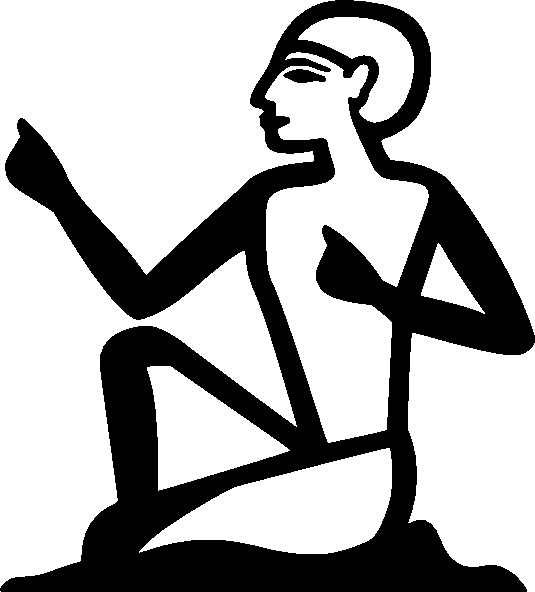
\includegraphics[height=1cm]{./hieroglyph-male.pdf} und 
\includegraphics[height=1cm]{./hieroglyph-female.pdf} Frau.

\vspace{1ex}

Namen werden in \enquote{Kartuschen} geschrieben: \cartouche{\pmglyph{K:l-i-o:p-a-d:r-a}}~
\includegraphics[height=0.6cm]{./hieroglyph-female.pdf}

\end{document}